% 03-data-exploration-and-preprocessing-appendix.tex

% \vspace{-1.1cm}

% Section Title
\section{DATA EXPLORATION AND PRE-PROCESSING}

    % Main Content

    This appendix contains additional plots and visualizations related to the data exploration and pre-processing phase of the analysis. The figures are grouped into subsections based on their thematic relevance.

    \subsection{Temporal Analysis of Attacks}

        This subsection presents visualizations related to the temporal distribution of SSH attacks, including trends over hours, days, months, and years.

        \subsubsection{Attack Frequency by Hour \\}
        
            The plot shows the distribution of SSH attacks across different hours of the day. It reveals specific hours when attack activity peaks, which could indicate targeted times for malicious activities. Understanding these patterns can help in implementing time-based security measures.
            
            \vspace{-0.1cm}

            \begin{figure}[H]
                \centering
                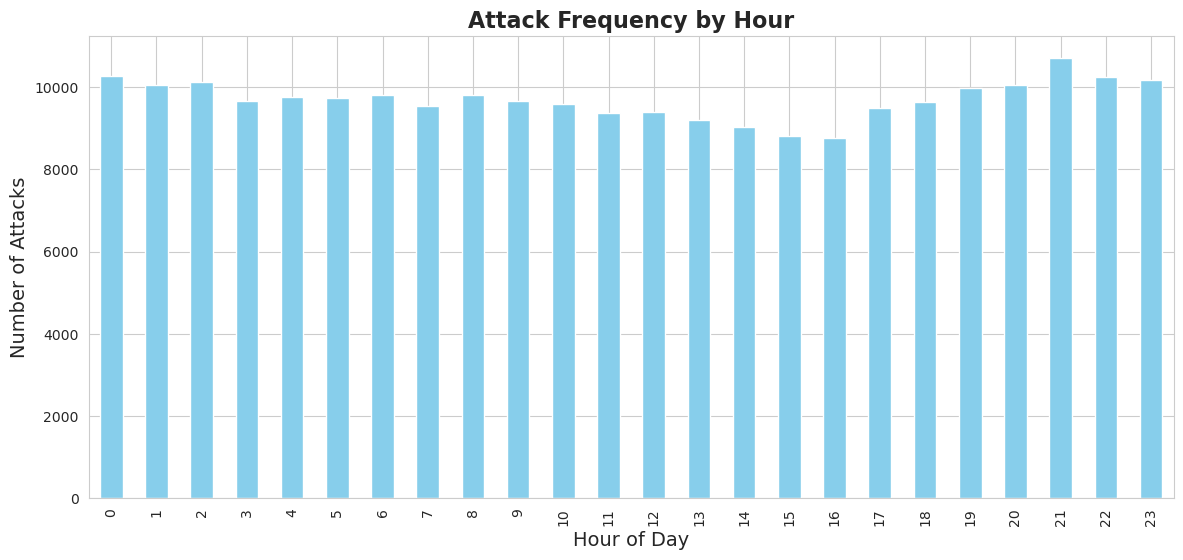
\includegraphics[width=0.7\textwidth]{../figures/plots/section1/attack_frequency_by_hour.png}
                \caption{Distribution of SSH attacks by hour of the day. The plot highlights peak hours during which attacks are most frequent.}
                \label{fig:attack_frequency_by_hour}
            \end{figure}

        \subsubsection{Attack Frequency by Month \\}
        
            This plot illustrates the distribution of SSH attacks across different months. It highlights seasonal trends, showing months with higher attack frequencies. Such insights can be useful for anticipating periods of increased security threats and allocating resources accordingly.

            \begin{figure}[H]
                \centering
                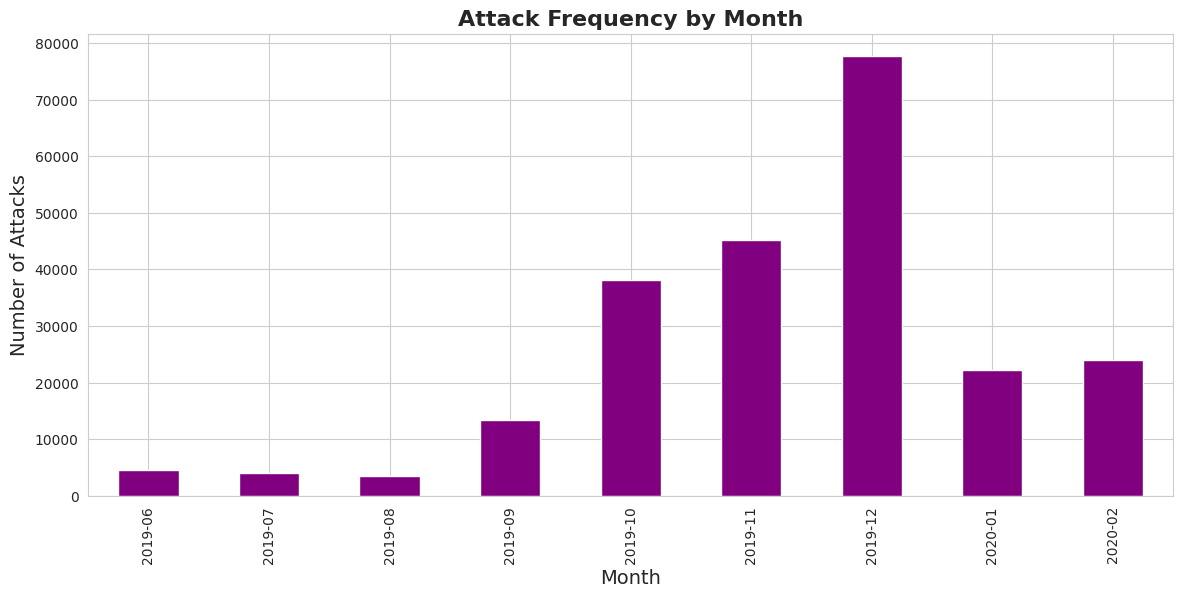
\includegraphics[width=0.7\textwidth]{../figures/plots/section1/attack_frequency_by_month.png}
                \caption{Distribution of SSH attacks by month. The plot reveals seasonal trends in attack frequency.}
                \label{fig:attack_frequency_by_month}
            \end{figure}

        \subsubsection{Attack Frequency by Year \\}
        
            The plot compares the frequency of SSH attacks between the years 2019 and 2020. It provides a clear view of how attack patterns have evolved over time, indicating whether there has been an increase or decrease in malicious activities. This information is crucial for understanding long-term trends and evaluating the effectiveness of security measures.

            \begin{figure}[H]
                \centering
                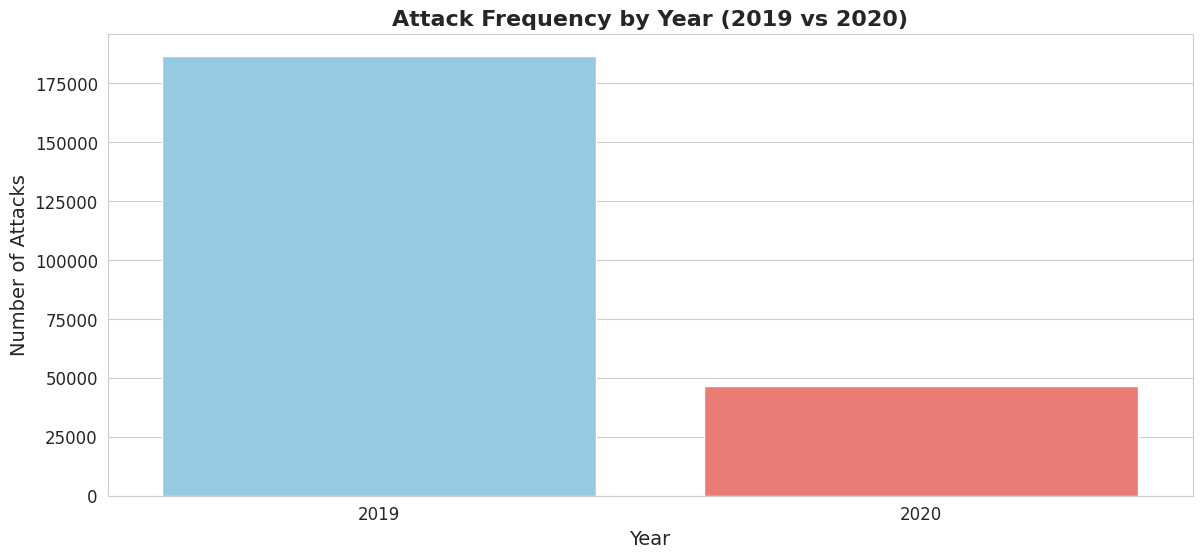
\includegraphics[width=0.7\textwidth]{../figures/plots/section1/attack_frequency_by_year.png}
                \caption{Distribution of SSH attacks by year. The plot shows the overall trend of attacks over multiple years.}
                \label{fig:attack_frequency_by_year}
            \end{figure}
            
        \subsubsection{Temporal Series of SSH Attacks \\}
        
            This time series plot provides a detailed view of SSH attack patterns over the entire dataset. It captures fluctuations in attack frequency, highlighting periods of heightened activity. Such a comprehensive view is essential for identifying anomalies and understanding the overall dynamics of SSH attacks.

            \begin{figure}[H]
                \centering
                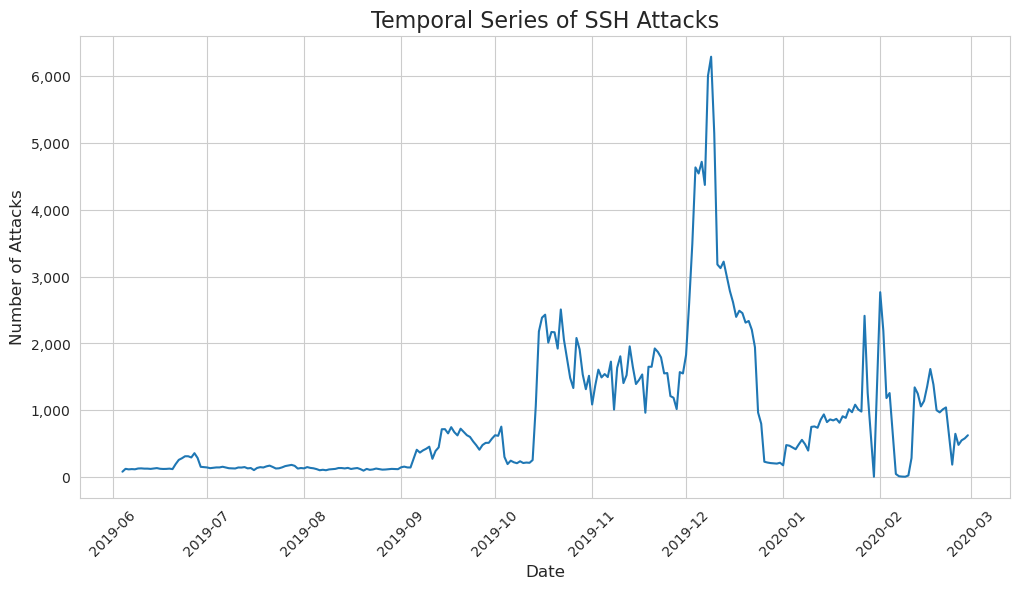
\includegraphics[width=0.7\textwidth]{../figures/plots/section1/temporal_series_of_ssh_attacks.png}
                \caption{Time series plot of SSH attacks over the entire dataset. The plot provides a comprehensive view of attack patterns over time.}
                \label{fig:temporal_series_of_ssh_attacks}
            \end{figure}

    \subsection{Intents Over Timestamps}

        This subsection explores the relationship between attack intents and their timestamps.

        \subsubsection{Intents Over Timestamps \\}
        
            The plot visualizes the distribution of different attack intents over time. It categorizes intents such as Defense Evasion, Harmless, Impact, Discovery, Persistence, Execution, and Others. By analyzing this plot, we can identify which intents are more prevalent at specific times, helping to prioritize security measures based on the nature of the threats.

            \begin{figure}[H]
                \centering
                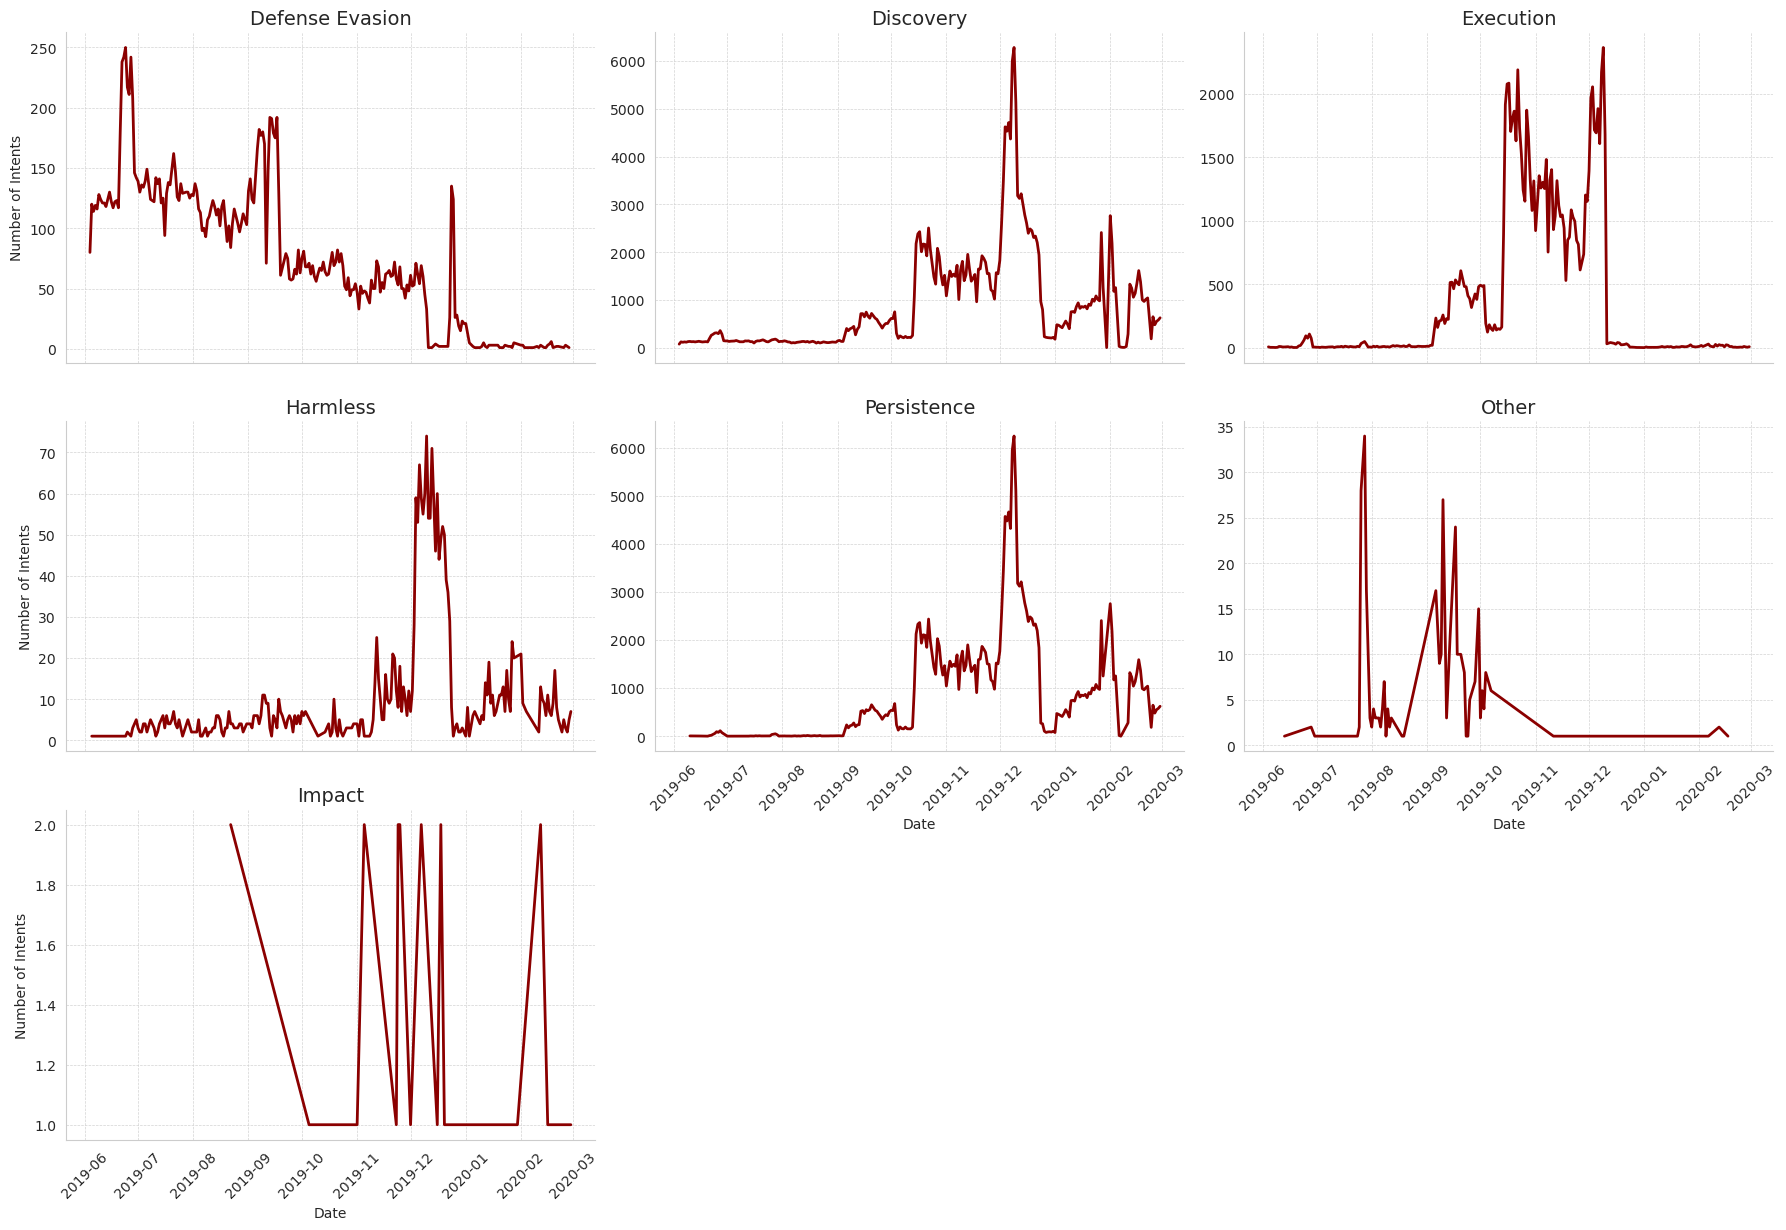
\includegraphics[width=0.85\textwidth]{../figures/plots/section1/intents_over_timestamps.png}
                \caption{Visualization of attack intents over timestamps. The plot provides insights into the temporal patterns of different attack intents.}
                \label{fig:intents_over_timestamps}
            \end{figure}
